\documentclass[a4paper,man,natbib]{apa6}

\usepackage[english]{babel}
\usepackage[utf8x]{inputenc}
\usepackage{amsmath}
\usepackage{graphicx}
\usepackage[colorinlistoftodos]{todonotes}
\usepackage{apacite}

\title{The use of non-linear programming in diversifying a financial portfolio}
\shorttitle{Non-linear GRG2 for portfolio diversification}
\author{Nelson Corrocher}
\affiliation{Harrisburg University}

\abstract{The purpose of this study is to apply a technique of non-linear optimization called Generalized Reduced Gradient (GRG2), to increase the diversification of a financial portfolio. One widely used risk-return measure for investment portfolios is the Sharpe-Ratio(SR) and by finding right proportions of investment products (IP) composing the portfolio, it is possible to obtain a greater SR than any standalone products. In this paper, historical prices of only six IPs (Google Stock, Gold, Crude, Real Estate, Brazilian Currency and S\&P 500 Index) were collected and used to demonstrated the validity of the approach, but the method can be extended to include any number of IPs. The computations were done in Microsoft Excel due its simplicity of use, immediate scalability in adding new products and the stability and maturity of its implementation of the GRG2 algorithm, but the approach was detailed enough so that any system with similar capabilities could be used.}

\begin{document}
	\maketitle
	
	\section{Introduction}
	The objective of this paper is to detail the process of using the non-linear optimization method of Generalized Reduced Gradient (GRG2) to optimize the risk-returns of financial portfolios.
	Before detailing the approach, however, it is necessary to state the problem, how it can be modeled, what is GRG2, how to apply it to the problem and how to measure the results. These questions will be the answered in the remaining of this paper.
	Even if the reader is not a competent financial analyst, it should be common knowledge that financial institutions offer different types of IPs for both individuals and businesses. Stocks, mutual funds, hedge funds and even the savings account are just a small fraction of all available IPs. With all these options, it is only natural to try to find the ones providing the best benefit.
	There are many ways used to measure and compare IPs and such subject would easily fill up an entire book. The scope of this paper, however, analyzes one specific and extensively used measure called \textbf{Sharpe-Ratio}, which will be the target of the optimization. In simple terms, the Sharpe-Ratio measures the risk-return of a portfolio, that is, how much return you can get for a certain amount of risk. In this context, \textbf{"return"} can be defined as the percentage one can get over an invested capital over a certain period of time and \textbf{"risk"} (or "volatility") is defined as the statistical variance that the investment showed over the same period of time. Now, it is possible to equate the Sharpe-Ratio in terms of these two definitions:
	\begin{equation}
	\text{Sharpe-Ratio} = \frac{(r_p - r_f)}{\alpha_p}
	\end{equation}
	where $r_p$ is the investment return, $r_f$ the risk-free rate and $\alpha_p$ the investment standard deviation (the squared root of variance). The risk-free rate is just how much return one can get without any risk (almost) and is usually measured by the interest paid by Treasure Bills with three months term. In summary, the lower the risk and the higher the return, the higher the SR. The higher the SR, the better the investment.
	With the SR defined, it remains the need to specify how it can be optimized and for this task, the concept of diversification will be addressed. While most readers would have heard that diversification is key to reduce risk in an investment, it is often unclear how it works. Diversification means combining different IPs in a way to reduce total volatility (a.k.a. risk) of the portfolio. The mathematical explanation of how it works is not part of the scope of this paper, but it can be showed that by combining $n$ IPs in a portfolio, the expected return and total volatility would be given by equations (2) and (3), below:
	\begin{equation}
	r_p = \sum_i x_ir_i
	\end{equation}
	with $x_i$ being the weight of the i-th investment on the portfolio and $r_i$ being the expected return from the i-th investment, and
	\begin{equation}
	\alpha_p = \sqrt{\sum_i\sum_j x_ix_jCov(r_i,r_j)}
	\end{equation}	
	with $x_i$ and $x_j$ being the weights of two investments $i$ and $j$ and $Cov(r_i,r_j)$ the covariance between the returns of the investments $i$ and $j$. As it can be noticed, the less relation two investments returns have, the smaller the covariance, and thus, smaller the denominator in the SR. The relation between two investments is determined by how much their returns are affected by the same events. Thus, the lower the relation, the lower the combined variance, or risk. This is, in summary, the concept diversification and the explanation of how it works. A more detailed explanation can be found in Chapter 11 of \cite{berk2014corporate}.
	Equations (1), (2) and (3) combined will make the basis for the formulation of the system of equations, or constraints, that the GRG2 algorithm will be applied upon in the next section. 
	But what about GRG2? GRG2 is a non-linear programming algorithm proposed by \cite{lasdon_fox_ratner_1974} and the most widely algorithm used today. A non-linear programming allows the numerical solving of a system of non-linear inequalities, required for solving the method proposed in the next section.  
	One final note before moving to the next section is that, as equation (3) shows, the time-complexity of the calculations grows quadratically to the number of IPs composing the portfolio, making manual calculations unfeasible for large numbers of IPs.
	\clearpage

	\section{Methodology}
	\subsection{Data collection}
	For this study, six financial products (plus the risk-free rate) with freely available historical prices were used. The list below show each product and its respective source of information:
	\begin{itemize}
		\item Gold \cite{gold_s};
		\item Crude Oil \cite{crude_s};
		\item Real Estate \cite{reit_s};		
		\item Google Stocks \cite{goog_s};
		\item Brazilian Currency \cite{bzf_s};
		\item S\&P 500 Index \cite{vfinx_s};
		\item Treasury Bill (risk-free rate) \cite{riskfree_s};
	\end{itemize}
	The collected data contained either price or the rate of return for a certain period, allowing the standardization of rates of returns and period. In this study, monthly rate-of-returns starting from January 2010 were used. By subtracting the risk-free rate from the rate-of-return for each IP, the data for calculating variance and average rate-of-return was generated.
	Next, for each IP, mean rate-of-return, standard deviation and SR were calculated. Lastly, correlation matrix between all IPs. This first three steps are trivial in excel by use =MEAN(), =STDEV.P() and the quotient between the two for SR and are shown in figure~\ref{fig:figure 1}. The correlation matrix was generated using the Data Analysis plug-in, Correlation function, shown in figure~\ref{fig:figure 2}.

	\subsection{Modeling}
	With the inputs prepared, the following procedure was to equate the problem in a system of inequalities so that GRG2 could be applied. To simply the explanation, from now on, the rate-of-return minus the risk-free rate of an IP will be referred as $R_p$ instead of $r_p$ so that the risk-free rate could be eliminated the inequalities.
	\begin{flalign}
	MAX:&\frac{\sum_i x_ir_i}{\sqrt{\sum_i\sum_j x_ix_jCov(r_i,r_j)}}&
	\end{flalign}
	is the target equation we want to maximize, with $x_i$ being the variables to be adjusted.
	The goal is to get the weights that would maximize the final portfolio SR. The only additional constraint is that the total weights of the portfolio have to be equal to 100\%:
	\begin{flalign}
	&\sum_i x_i = 1&
	\end{flalign}
	\textbf{NOTE:} The $x_i$ variables CAN have a negative weight, which in financial terms mean "shorting" the IP, which is a slightly more sophisticated transaction that involves borrowing, selling then re-buying the asset at a later period, expecting the price to go down. However, this transaction can affect the outcome by including artificial risks created by brokers and operators that can't be easily modeled in the Sharpe-Ratio. In such case, one possible refinement could be to limit $x_i$ by setting up greater than 0 or some lower value, depending on the operator's criteria, $x_i$ > $u$, with $u$ being some restriction imposed by trading officer.
	Since the data in real world is not perfect, some products may show incorrect of floating rates-of-returns or variances and its inclusion in portfolio could lead to strange results, like arbitrage opportunities. To avoid such situation, another refinement could be to set all $x_i$ > -1.
	The final step is to set all this information in an excel spreadsheet (many ways exist, one possible model is shown in the Appendix), call the excel plug-in Solver, mapping the inputs and selecting GRG2 nonlinear as the algorithm. The algorithm will change the values of the cells containing the weights, trying to make the target function converge to a maximum value. After the execution, the variating cells will contain the optimal weights for each IP.
	
	\section{Results and Analysis}
	The results from the execution of the algorithm are shown on figure~\ref{fig:figure 3}. It can be seems that by optimizing the weights on the portfolio, the Sharpe-Ratio was increased to 0.34 and the portfolio mean return per month is estimated to be 0.9\% while the volatility (technically, the square of it) is about 2.63\%. Comparing this results to the ones from figure 1, it can be seem that the new SR is higher than that of any individual IP.
	One question regarding the portfolio optimality after the GRG2 algorithm calculated the weights, would be that, even though the SR is higher, the returns are not as high as those of some products. For example, Google Stock offers a return of 1.45\% per month but with a volatility of 7.14\%. The optimal portfolio provides only a return of 0.90\% per month but with a volatility of 2.63\%. What if the investor wanted Google's stocks rate of return? Instead of changing the constraints and re-running the algorithm, it is possible to borrow money and to invest it in the portfolio (technique called leverage). Leverage increase returns but also the risks. To simplify this demonstration, assume it is possible to borrow and lend in the same risk-free rate (not true, but can be proven that it won't change the SR optimality). With this assumption, the risk-return relation is linear and by assuming the same risk as Google Stock, that of 7.14\%, the return on the leveraged portfolio would be $\dfrac{0.90}{2.63} * 7.14 = 2.44$. So, by assuming the same risk as Google Stock, one would be getting 2.44\% return instead of 1.45\%. This logic also works in reverse: if the investor wants a lower risk instead, he could invest a portion of his money in the risk-free rate, reducing returns but also the risk. 

	\section{Conclusion}
	By comparing the optimal portfolio SR vs each IP, it becomes clear that applying the GRG2 method for optimization not only improve returns effectively, but also cheaply. Decades ago, when computation resources were expensive and rare, it was unfeasible to manually calculate the optimal SR for more than 10 products and short-cuts were taken for approximations. If the investors requirements changed, the portfolio weight would have to be recalculated again. By finding the mathematical optimal value for the portfolio, no recalculations are needed after the optimal SR is found (except in the case the risk/return of the composing products change).
	
	\bibliographystyle{apacite}
	\bibliography{bibliography}
	
	% Commands to include a figure:
	\begin{figure}
	\centering
	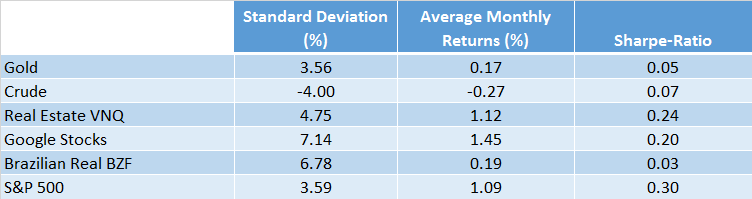
\includegraphics[width=0.8\textwidth]{basic_stat.png}
	\caption{\label{fig:figure 1}Basic statistics from investment products}
	\end{figure}
	\begin{figure}
	\centering
	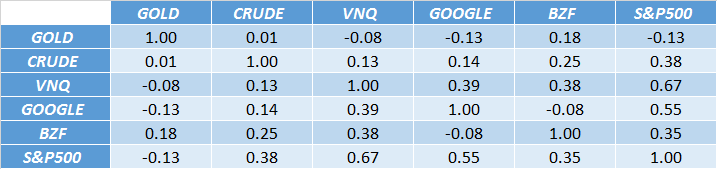
\includegraphics[width=0.8\textwidth]{correl_matrix.png}
	\caption{\label{fig:figure 2}Correlation matrix between rate of returns of investment products}
	\end{figure}
	\begin{figure}
	\centering
	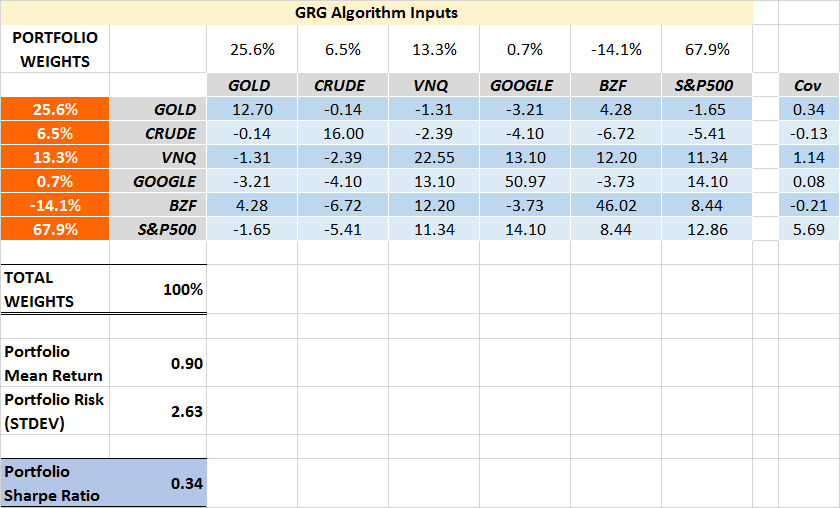
\includegraphics[width=0.8\textwidth]{results.png}
	\caption{\label{fig:figure 3}Results found by the GRG2 algorithm}
	\end{figure}
	
\end{document}